%%\documentclass[t]{beamer}
\documentclass[t,handout]{beamer}

\usepackage{graphicx}
\usepackage{pgf}
\usepackage{epsfig}
\usepackage{psfrag}
\usepackage[english]{babel}
\usepackage{hyperref}

\usepackage{listings}
\usepackage{courier}
\usepackage{color}

\lstset{
	language=Ruby,
	basicstyle=\footnotesize\ttfamily\color{black},
	commentstyle = \footnotesize\ttfamily\color{red},
	keywordstyle=\footnotesize\ttfamily\color{blue},
	stringstyle=\footnotesize\ttfamily\color{black},
%	columns=fixed,
%	numbers=left,    
	numberstyle=\tiny,
	stepnumber=1,
	numbersep=5pt,
	tabsize=1,
	extendedchars=true,
	breaklines=true,            
	frame=b,         
	showspaces=false,
	showtabs=true,
	xleftmargin=6pt,
	framexleftmargin=6pt,
	framexrightmargin=2pt,
	framexbottommargin=4pt,
	showstringspaces=false      
}

\lstloadlanguages{
         Ruby,HTML
}
 %\DeclareCaptionFont{blue}{\color{blue}}

\newcommand{\asgn}{\mbox{$\bf\leftarrow$ }}  %pseudocode assignment stmt
\newcommand{\comt}{\mbox{$\; \rhd$ \ }}  %pseudocode comment

\graphicspath{{images/}} % Figures path - used in graphicx

%\selectcolormodel{cmyk}

\mode<presentation>

\usetheme{Warsaw}

\title[Module 5, Lecture 2]{ECE 495/595 -- Web Architectures/Cloud Computing}
\subtitle{Module 5, Lecture 2: Web Application Security -- Authentication}

\author[\copyright \ 2012 C. C. Lamb]{Christopher Lamb Ph.D, CISSP, TCEA}
\date{}
\institute[University of New Mexico]{\large University of New Mexico}

\titlegraphic{
\begin{figure} 
\hspace{2cm}

\includegraphics[width = 4in]{ECE-UNM-logo.pdf}
\end{figure}}

\begin{document}

\begin{frame}
\titlepage
\end{frame}

% This command will make the logo appear on all frames excluding the title frame.
\logo{
\includegraphics[width = 0.75in]{UNM.pdf}}

%\begin{frame}
%\frametitle{Overview}
%\tableofcontents 
%\end{frame}

\section{What is Capistrano?}
\begin{frame}
\frametitle{What is Capistrano?}
\end{frame}

\section{Why use it?}
\begin{frame}
\frametitle{Starting out...}

\includegraphics[width = 4in]{cap-app.pdf}
\transfade
\end{frame}

\begin{frame}
\frametitle{...where to put it?}

\includegraphics[width = 4in]{cap-app-srv.pdf}
\transfade
\end{frame}

\begin{frame}
\frametitle{...and how to store stuff?}
\begin{center}
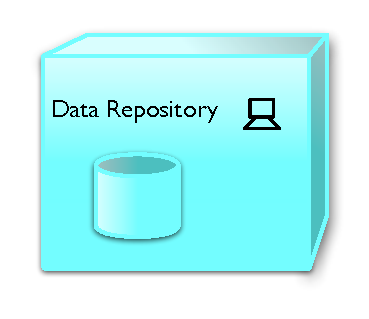
\includegraphics[width = 3in]{cap-data-repo.pdf}
\end{center}
\transfade
\end{frame}

\begin{frame}
\frametitle{...now linking it together...}
\begin{center}
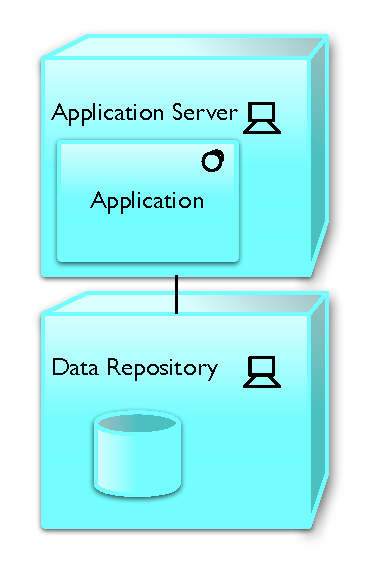
\includegraphics[width = 1.75in]{cap-stack.pdf}
\end{center}
\transfade
\end{frame}

\begin{frame}
\frametitle{...and this is how you manage it.}
\begin{center}
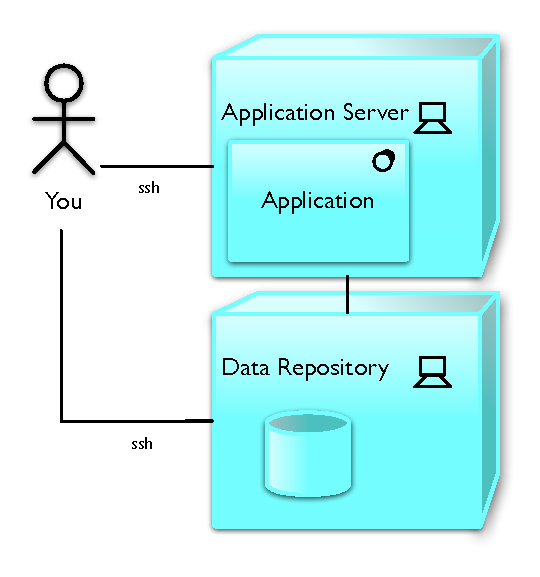
\includegraphics[width = 2.5in]{cap-stack-you.pdf}
\end{center}
\transfade
\end{frame}

\begin{frame}
\frametitle{Is this sufficient?}
Well, probably okay for:
\begin{small}
\begin{itemize}
\item School
\item Departments
\item Small organizations
\end{itemize}
\end{small}
But honestly, not very real world.  Systems with any kind of availability requirements or volume usually have:
\begin{small}
\begin{itemize}
\item More systems
\item Specialized systems
\item More providers
\end{itemize}
\end{small}
\begin{center}
{\bf Really? Well, why not?}
\end{center}
\end{frame}

\begin{frame}
\frametitle{Typical small deployment...}
\begin{center}
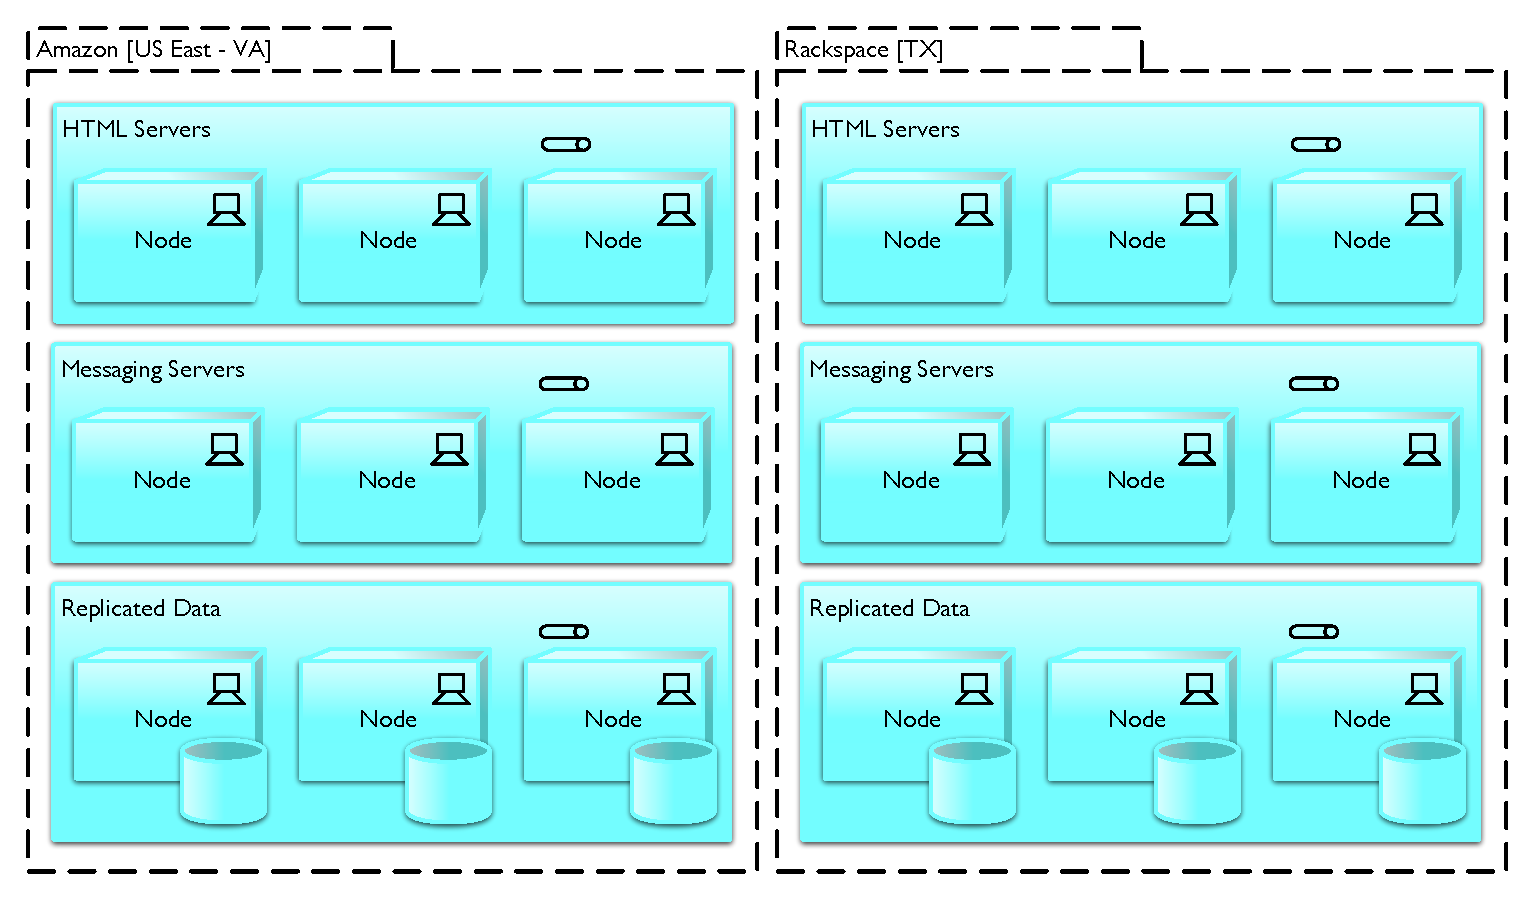
\includegraphics[width = 4in]{cap-distributed.pdf}
\end{center}
\transfade
\end{frame}

\begin{frame}
\frametitle{...and you're responsible for it.}
\begin{center}
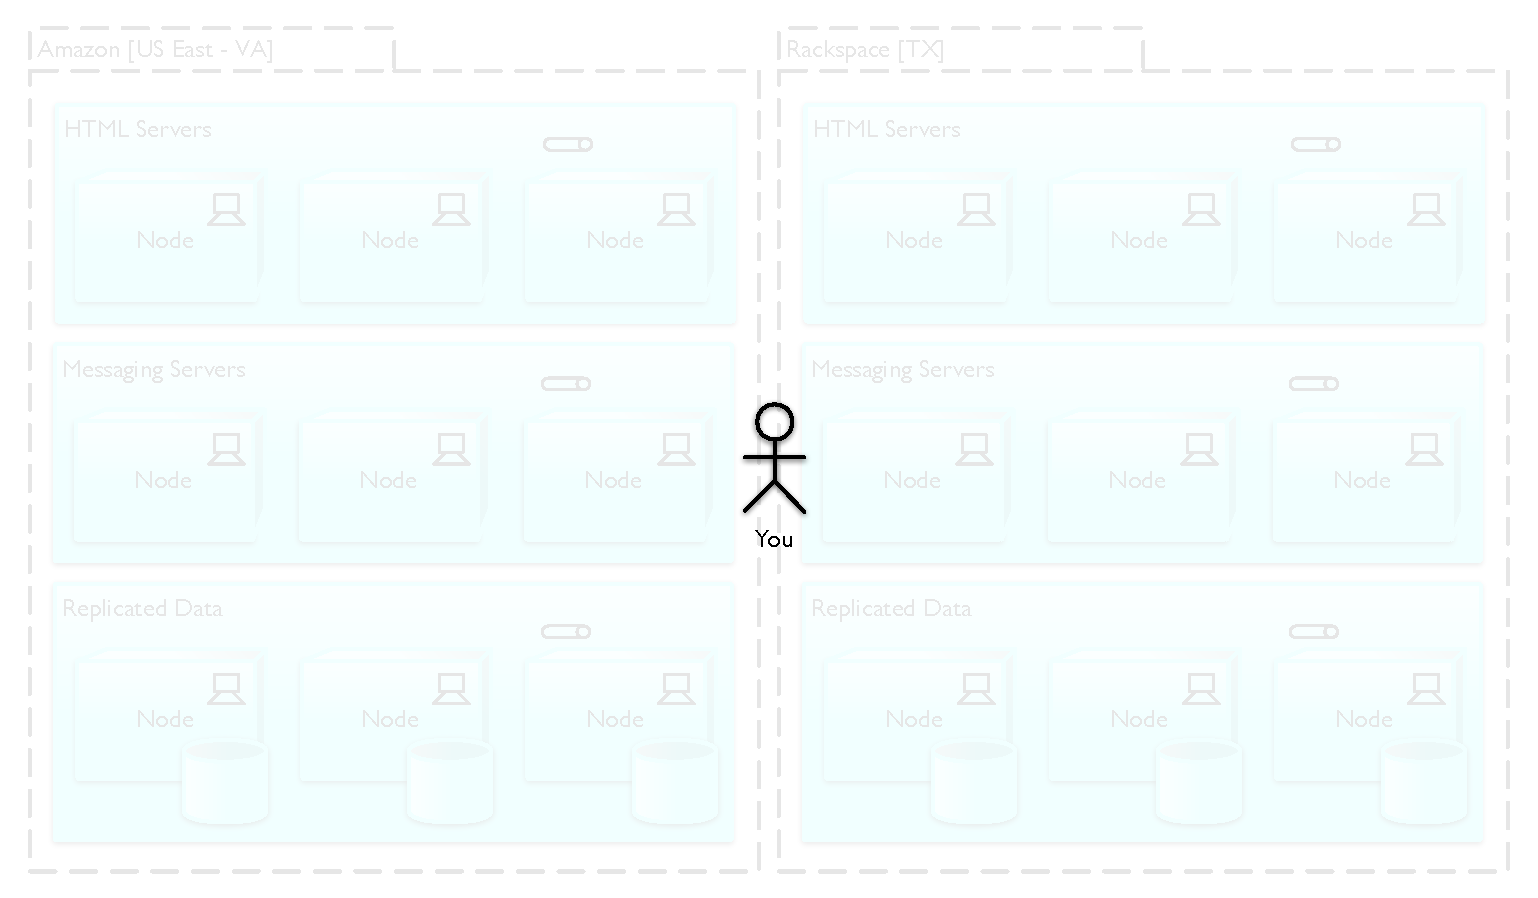
\includegraphics[width = 4in]{cap-distributed-you.pdf}
\end{center}
\transfade
\end{frame}

\end{document}


